\begin{itemize}[--]
	\item Package name should be the reverse domain name that you own (eg. com.example - you can't publish a project with this namespae)
	\item The target SDK is automatically assigned to the most recent version
	\item MinSDK must should balance a large audience with new features
	\item An \textbf{activity} serves as a presentation layer for our UI
	\item A \textbf{fragment} represents a behaviour or portion of our screen
	\item To create a new icon:
	\begin{enumerate}
		\item Right-click$\to$New$\to$Image Asset.
		\item Choose an image
		\item Overwrite ``ic\_launcher''
	\end{enumerate}
	
	\item Android Stack:
	\begin{itemize}[--]
		\item Application Layer
		\item Application Framework
		\item C/C++ Libs \& Android Runtime
		\item Linux Kernel
	\end{itemize}

	\item Gradle is the build toolkit for handling dependencies and building into byte code, resources, and manifest
	\begin{center}
		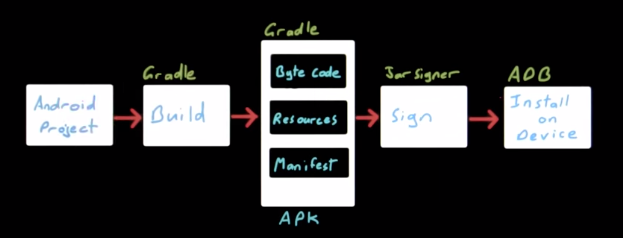
\includegraphics[scale=0.7]{sections/1/gradle_workflow.png}
	\end{center}

	\item The ``res'' file contains all the resource files: layouts, values, images
	\item Fame, Linear, and Relative layout are basic view groups
	\item \textbf{Frame layout}: useful for simple layouts, with a single view or stack or views. Views are all algined against the frame boundaries only.
	\item \textbf{Linear layout}: perfect for stacking views vertically or horizontally, one after another. Only way to break-up display proportionally.
	\item \textbf{Relative layout}: sophisticated layout that allows the position of views relative to other views or the boundaries of the view
	\item \textbf{ScrollView} allows the ability to scroll through the content of the layout it contains
	\item \textbf{ListView} starts by filling the screen with views, and a few on either end to assure no loading on scroll.
	\item Each view is recycled to save memory when it's moved off screen, which is how all \textbf{AdapterView} objects behave
	\begin{center}
		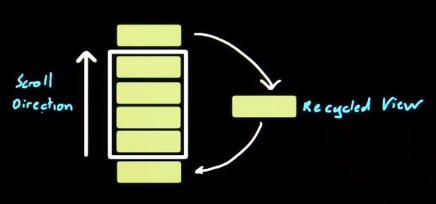
\includegraphics[scale=0.7]{sections/1/recycle.png}
	\end{center}

	\item An adapter then serves an interface for the data, managing location and creation (so memory is dealt with effectively)
	\begin{center}
		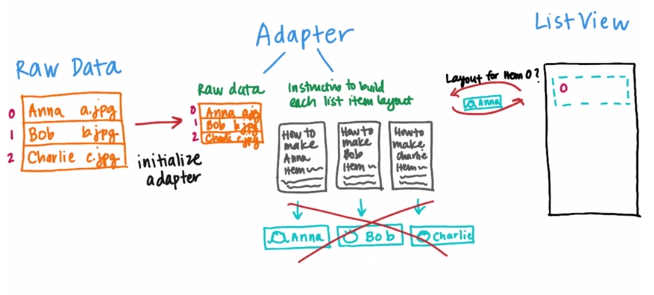
\includegraphics[scale=0.6]{sections/1/adapter.png}
	\end{center}

	\item For the sunshine data, which is in array, we'll use an ArrayAdapter, with the paramters:
	\begin{itemize}[--]
		\item Context: global info about app environment, including access to system servcies: \texttt{getActivity\(\)}
		\item ID of the list item layout: resource id of layout: \texttt{R.layout.list\_item\_forecast}
		\item ID of text view: resource id of UI: \texttt{R.id.list\_item\_forecast\_textview}
		\item List of data: data object \texttt{weekForecast}
	\end{itemize}

	\item ID's aren't required if you don't need a reference to the View/ViewGroup
	\item View/ViewGroup's are referenced via the \texttt{findViewById(ID)} function, with the parameter being the ID of the view in question
	\item It finds the view by searching through the XML layout's inflated view hierarchy
	\begin{center}
		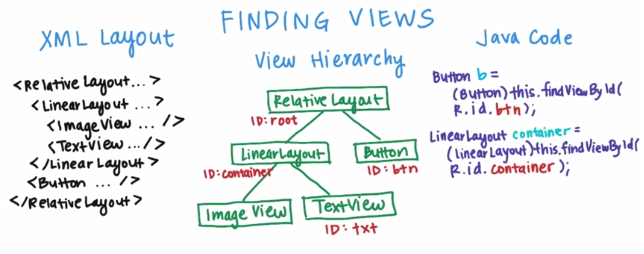
\includegraphics[scale=0.6]{sections/1/views.png}
	\end{center}

	\item You can search through subtrees of the hierarchy by calling the \texttt{findViewById} for that particular viewgroup: \texttt{container.findViewByID(ID)}
	\item 
\end{itemize}